\chapter{Name Services}
\begin{multicols*}{2}

\noindent Names identify resources in a \emph{location-independent} fashion. Addresses identify resources in a \emph{location-dependent} fashion.\\

\noindent Name service does translation between names and addresses. Name resolution is the conversion process from names to addresses.\\

\noindent Main requirements of name services:
\begin{itemize}
  \item Scalability: to handle arbitrary number of names and to serve an arbitrary number of administrative organizations over long lifetime
  \item Reliability: name services should not fail frequently
  \item Performance: name resolution should have short response time
\end{itemize}

\noindent Name space is the collection of all valid names. Name space requires a syntatic definition. Name space can have hierarchical structure or flat structure, but hierarchical name space has better scalability than flat name space.

\section{Name Resolution Process}

\noindent Physically, the resolution process may involve more than on name server because the mapping may not be available at every name server.\\

\noindent Method 1: Iterative Client-controller Navigation. A client iteratively contacts a group of name servers to resolve a name. However, this method has high communication cost if name servers are located far away.\\

\noindent Method 2: Non-recursive Server-controller Navigation. A name server coordinates the name resolution process iteratively or multicast on behalf of a client.\\

\noindent Method 3: Recursive Server-controller Navigation. If a name server does not have the name mapping, it contact another name server, and this procedure continues recursively until the name is resolved. The caching results is more effective, but it put higher performance demand on each name server.

\section{Domain Name System}

\noindent To meet requirements of name services, DNS uses:
\begin{itemize}
  \item Scalability: hierarchical name space
  \item Reliability: use replication
  \item Performance: use caching
\end{itemize}

\subsection{Hierarchical Name Space}

\begin{center}
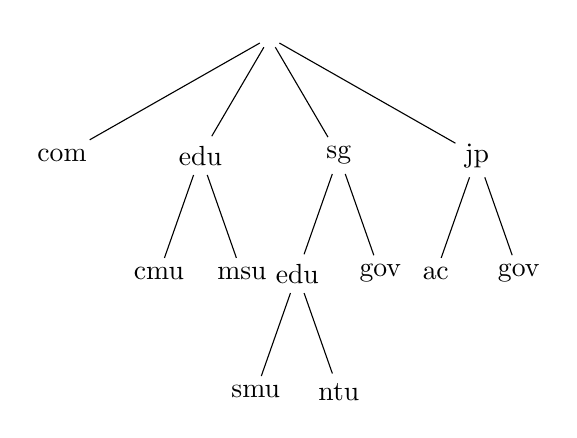
\begin{tikzpicture}[
recnode/.style={rectangle, draw=white, thin},
level 1/.style={sibling distance=5em},
level 2/.style={sibling distance=3em},
]
%Nodes
\node[recnode,draw](Top){}
    child {node[recnode,draw](com){com} edge from parent[-]}
    child {node[recnode,draw](edu){edu} edge from parent[-]
      child {node[recnode,draw](cmu){cmu} edge from parent[-]}
      child {node[recnode,draw](msu){msu} edge from parent[-]}
    }
    child {node[recnode,draw](sg){sg} edge from parent[-]
      child {node[recnode,draw](edu2){edu} edge from parent[-]
        child {node[recnode,draw](smu){smu} edge from parent[-]}
        child {node[recnode,draw](ntu){ntu} edge from parent[-]}
      }
      child {node[recnode,draw](gov){gov} edge from parent[-]}
    }
    child {node[recnode,draw](jp){jp} edge from parent[-]
      child {node[recnode,draw](ac){ac} edge from parent[-]}
      child {node[recnode,draw](gov2){gov} edge from parent[-]}
    }
;
\end{tikzpicture}
\end{center}

\noindent DNS uses a decentralized design, i.e no single server is responsible for all names. The entire name spaces is partitioned among a large group of name servers. Each server holds authoritative mappings for the names in one or more domains. \\

\noindent Each mapping contains domain name, time-to-live, class, type and value. The information held in DNS servers are:
\begin{itemize}
  \item Mappings between names and IP addresses for the local domain
  \item Names and addresses of all name servers in local domain, sub-domains, and root name servers
\end{itemize}

\noindent Type of mapping:
\begin{itemize}
  \item A-type record maps a computer name to its IP address
  \item CNAME-type record maps an alias to its canonical name
  \item NS-type record specifies authoritative name servers. Each NS-record is accompanied by an A-type record.
  \item MX-type record gives preferences and domain names of mail hosts
\end{itemize}

\subsection{Replication for Reliability}

\noindent Authoritative mappings of each domain must be held by at least two name servers, i.e. the primary server and secondary servers. Secondary servers periodically check with the primary server to see whether their stored mappings are up-to-date. \\

\noindent DNS uses a simple request-reply protocol between clients and name servers based on UDP. DNS primarily uses a combination of iterative client-controlled navigation and non-recursive server- controlled navigation. 

\subsection{Caching for Performance Improvement}

\noindent Results of name resolution may be cached by clients and name servers. Clients and name servers always consult their caches before sending queries to other servers for name resolution. \\

\noindent However, caching introduces inconsistency problem. Query answers returned from cached mappings may be out-of-date. The consistency problem can be addressed by timeouts (time-to-live values).

\end{multicols*}
